

\subsection{Resultados de la Velocidad de Backup en Diferentes Tamaños de Archivos}

En este apartado se presentan los resultados obtenidos al medir la velocidad de backup para diferentes tamaños de archivos. La Figura \ref{fig:backup-velocidad-tamaño} muestra los tiempos de backup en función del tamaño del archivo.

\begin{figure}[H]
    \centering
    \includegraphics[width=0.8\textwidth]{backup_velocidad_tamaño.png}
    \caption{Velocidades de Backup para Diferentes Tamaños de Archivo}
    \label{fig:backup-velocidad-tamaño}
\end{figure}

\textbf{Descripción de los Datos:}
Los datos muestran que para archivos de hasta 100 MB, el tiempo de backup es prácticamente constante y muy bajo (menos de un segundo). Sin embargo, a medida que el tamaño del archivo aumenta a 1 GB y más, el tiempo de backup incrementa de manera significativa. Para archivos de 10 GB, el tiempo de backup llega a superar los 450 segundos.

\textbf{Análisis de Resultados:}
Los resultados indican una relación no lineal entre el tamaño del archivo y el tiempo de backup, observándose un crecimiento exponencial del tiempo de backup a medida que el tamaño del archivo aumenta. Este comportamiento sugiere que para tamaños de archivo pequeños, la sobrecarga inicial del sistema y la latencia no afectan significativamente el tiempo de backup. Sin embargo, para archivos más grandes, la cantidad de datos que se debe procesar y transferir domina el tiempo total de backup. Este crecimiento exponencial es esperable, dado que a medida que aumenta el tamaño del archivo, se incrementa también la cantidad de operaciones de entrada y salida, así como la carga de procesamiento requerida para manejar los datos.

\textbf{Incertidumbre de la Medida:}
También es importante destacar que la incertidumbre o el error en la medición del tiempo de backup crece con el tamaño del archivo. Esto se puede observar en las barras de error presentes en la gráfica, las cuales se vuelven más pronunciadas a medida que aumenta el tamaño del archivo. Esta creciente incertidumbre refleja las variaciones y posibles fluctuaciones en el rendimiento del sistema durante el proceso de backup, especialmente para archivos de gran tamaño.

\textbf{Importancia del Tamaño del Pool:}
El tamaño del pool de almacenamiento es un factor crítico en la eficiencia del backup. Un pool más grande puede manejar archivos grandes más eficientemente al distribuir la carga de trabajo entre más recursos. Sin embargo, si el pool es demasiado pequeño, puede convertirse en un cuello de botella, incrementando significativamente los tiempos de backup. Por lo tanto, es crucial dimensionar adecuadamente el pool de almacenamiento para asegurar una operación de backup eficiente y escalable.




%%%%%%%%%%%%%%%%%%%%%%%%%%%%%%%%%%%%%%%%%%%%%%%%%
\subsection{Resultados de la Velocidad de Backup de 1 GB en Diferentes Tamaños de Archivos de Fracción de 1 GB}

En este apartado se presentan los resultados obtenidos al medir la velocidad de backup para un archivo de 1 GB, dividido en diferentes tamaños de archivos más pequeños. La Figura \ref{fig:backup-velocidad1gb} muestra los tiempos de backup en función del tamaño de la fracción de archivo.

\begin{figure}[H]
    \centering
    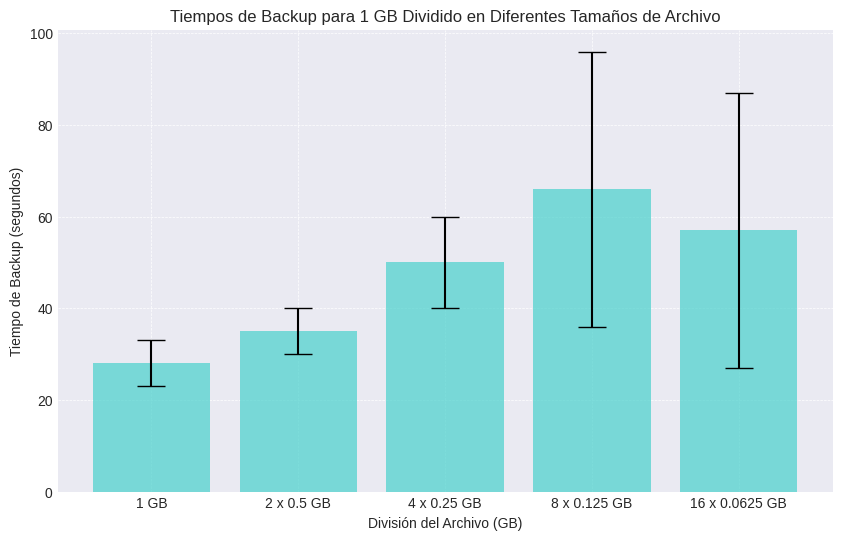
\includegraphics[width=0.8\textwidth]{backup_velocidad1gb.png}
    \caption{Tiempos de Backup para 1 GB Dividido en Diferentes Tamaños de Archivo}
    \label{fig:backup-velocidad1gb}
\end{figure}

\textbf{Descripción de los Datos:}
Los datos muestran que al dividir un archivo de 1 GB en fracciones más pequeñas, el tiempo de backup varía significativamente. Para un solo archivo de 1 GB, el tiempo de backup es de aproximadamente 28 segundos con una desviación estándar de ±5 segundos. Cuando se divide en dos archivos de 0.5 GB, el tiempo de backup aumenta a aproximadamente 35 segundos con una desviación estándar de ±5 segundos. Al dividirse en cuatro archivos de 0.25 GB, el tiempo de backup sube a unos 50 segundos con una desviación estándar de ±10 segundos. La división en ocho archivos de 0.125 GB resulta en un tiempo de backup de aproximadamente 66 segundos con una desviación estándar de ±30 segundos. Finalmente, la división en dieciséis archivos de 0.0625 GB muestra un tiempo de backup de unos 57 segundos con una desviación estándar de ±30 segundos.

\textbf{Análisis de Resultados:}
Los resultados indican que el tiempo de backup no aumenta linealmente con la división del archivo de 1 GB en fracciones más pequeñas. En cambio, se observa un aumento inicial del tiempo de backup cuando se pasa de un único archivo a varias fracciones, seguido de una mayor variabilidad en los tiempos de backup a medida que el número de fracciones aumenta. Esta variabilidad es notable en las barras de error, que se vuelven más pronunciadas a medida que disminuye el tamaño de cada fracción.

\textbf{Comportamiento Observado:}
La tendencia observada puede deberse a varios factores, incluyendo la sobrecarga administrativa asociada con el manejo de múltiples archivos y la mayor cantidad de operaciones de entrada y salida requeridas para procesar estos archivos más pequeños. La creciente incertidumbre en las mediciones para tamaños de fracción más pequeños sugiere que otros factores del sistema, como la latencia y la carga de procesamiento, tienen un impacto más pronunciado cuando se manejan múltiples archivos simultáneamente.


%%%%%%%%%%%%%%%%%%%%%%%%%%%%%%%%%%%%%%%%%%%%%%%%

\subsection{Resultados del Impacto de los Niveles de Compresión en la Compresión, Velocidad y Bytes Escritos}

En este apartado se presentan los resultados obtenidos al medir cómo los diferentes niveles de compresión (LZO y GZIP del 1 al 9) afectan la compresión, la velocidad de respaldo y los bytes escritos. A continuación se presentan y discuten los resultados obtenidos.

\begin{figure}[H]
    \centering
    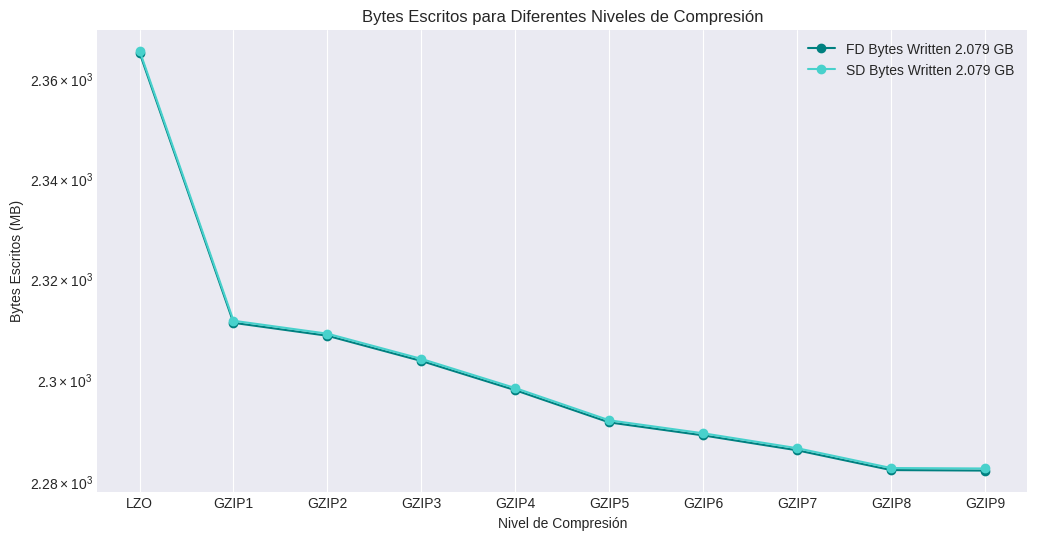
\includegraphics[width=0.8\textwidth]{bytes_escritos_archivo_grande.png}
    \caption{Bytes Escritos para Diferentes Niveles de Compresión (Archivo de 2.079 GB)}
    \label{fig:bytes_escritos_grande}
\end{figure}

\begin{figure}[H]
    \centering
    \includegraphics[width=0.8\textwidth]{bytes_escritos_archivo_pequeño.png}
    \caption{Bytes Escritos para Diferentes Niveles de Compresión (Archivo de 42 MB)}
    \label{fig:bytes_escritos_pequeño}
\end{figure}

\begin{figure}[H]
    \centering
    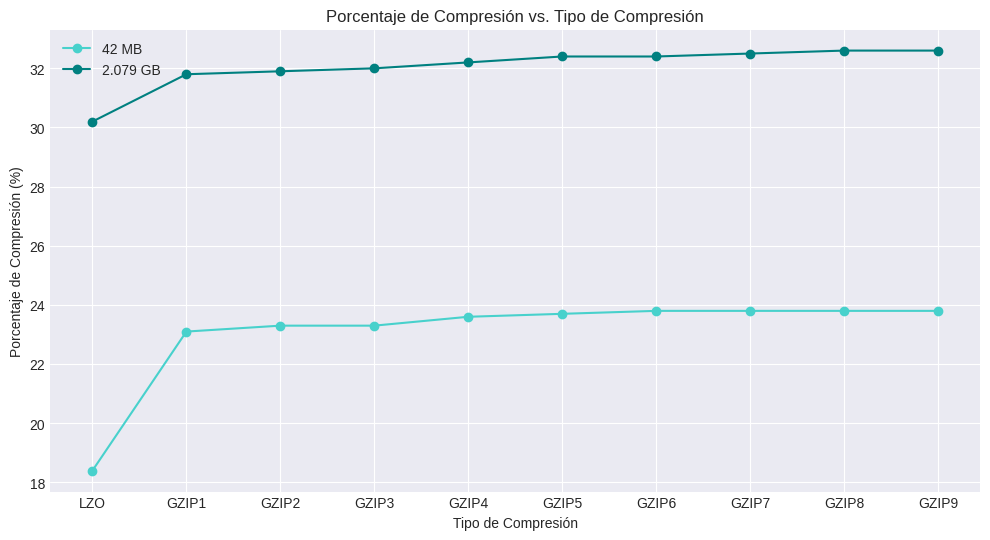
\includegraphics[width=0.8\textwidth]{porcentaje_compresion.png}
    \caption{Porcentaje de Compresión vs. Tipo de Compresión}
    \label{fig:porcentaje_compresion}
\end{figure}

\begin{figure}[H]
    \centering
    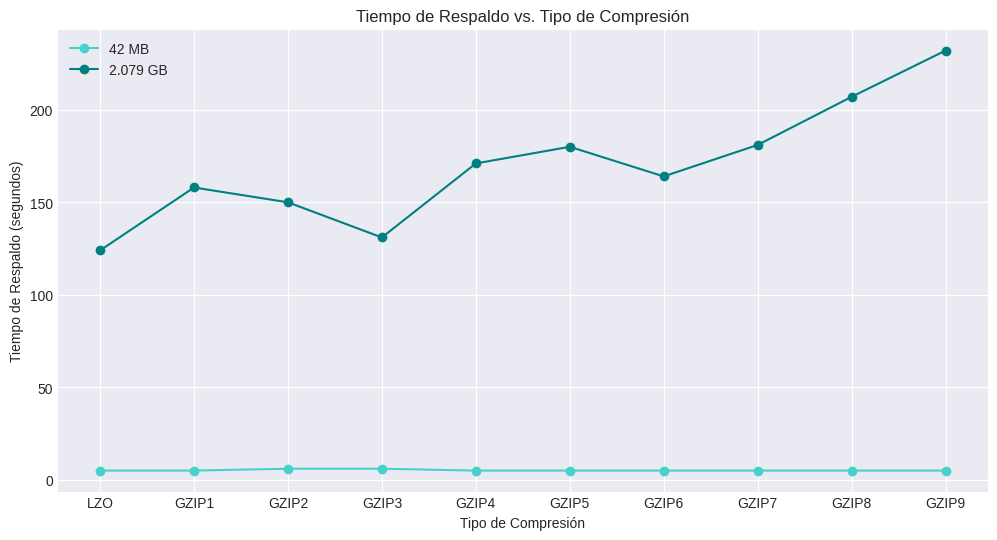
\includegraphics[width=0.8\textwidth]{tiempo_respaldo.png}
    \caption{Tiempo de Respaldo vs. Tipo de Compresión}
    \label{fig:tiempo_respaldo}
\end{figure}

\textbf{Bytes Escritos:}
La Figura \ref{fig:bytes_escritos_grande} y la Figura \ref{fig:bytes_escritos_pequeño} muestran los bytes escritos por el File Daemon (FD) y el Storage Daemon (SD) para un archivo de 2.079 GB y 42 MB, respectivamente, bajo diferentes niveles de compresión. Se observa que el uso de GZIP, incluso en su nivel más bajo (GZIP1), reduce significativamente la cantidad de bytes escritos en comparación con LZO. A medida que aumenta el nivel de compresión de GZIP, los bytes escritos continúan disminuyendo, aunque el decremento se vuelve menos pronunciado en los niveles más altos.

\textbf{Porcentaje de Compresión:}
La Figura \ref{fig:porcentaje_compresion} muestra el porcentaje de compresión alcanzado con LZO y diferentes niveles de GZIP para archivos de 42 MB y 2.079 GB. Los resultados indican que GZIP logra una mayor compresión que LZO. En particular, el porcentaje de compresión mejora ligeramente con niveles más altos de GZIP, aunque la diferencia se reduce a partir de GZIP6. Para los archivos más grandes, el porcentaje de compresión es consistentemente más alto en comparación con los archivos más pequeños.

\textbf{Tiempo de Respaldo:}
La Figura \ref{fig:tiempo_respaldo} presenta los tiempos de respaldo para los archivos de 42 MB y 2.079 GB bajo diferentes niveles de compresión. Se observa que el tiempo de respaldo aumenta con niveles más altos de compresión, especialmente para el archivo más grande. El tiempo de respaldo con LZO es significativamente menor que con GZIP, lo que sugiere que aunque GZIP proporciona una mejor compresión, lo hace a costa de un mayor tiempo de procesamiento.

\textbf{Análisis de Resultados:}
Los resultados muestran que la elección del algoritmo de compresión y su nivel tiene un impacto significativo en los bytes escritos, el porcentaje de compresión y el tiempo de respaldo. GZIP, especialmente en niveles más altos, ofrece una mayor compresión en comparación con LZO, pero con un incremento notable en el tiempo de respaldo. Esto sugiere que para optimizar la eficiencia de almacenamiento, GZIP es preferible, mientras que LZO puede ser más adecuado cuando el tiempo de respaldo es una consideración crítica.

%%%%%%%%%%%%%%%%%%%%%%%%%%%%%%%%%%%%%%%%%%%%%%%



\subsection{Resultados de los Tiempos de Restauración para los Distintos Tamaños de Archivos}

En este apartado se presentan los resultados obtenidos al medir los tiempos de restauración para diferentes tamaños de archivos. La Figura \ref{fig:tiempo-restauracion} muestra los tiempos de restauración en función del tamaño del archivo.

\begin{figure}[H]
    \centering
    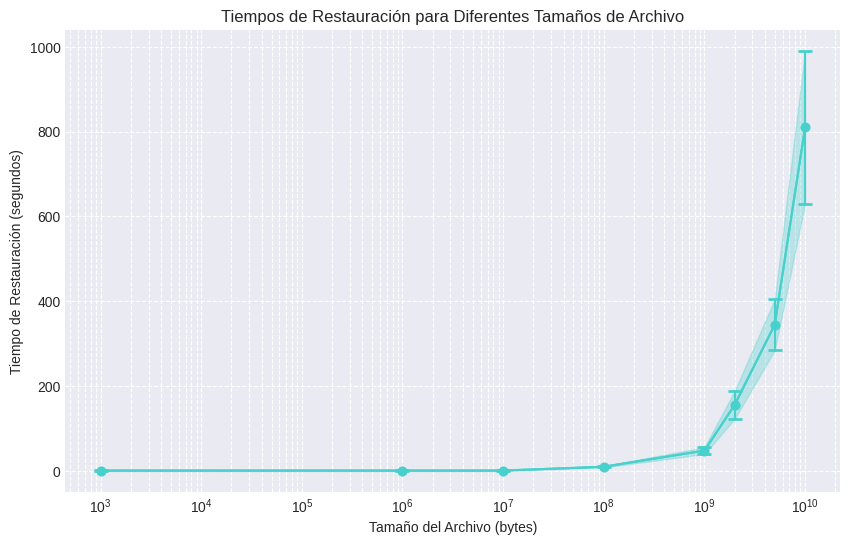
\includegraphics[width=0.8\textwidth]{tiempo_restauracion.png}
    \caption{Tiempos de Restauración para Diferentes Tamaños de Archivo}
    \label{fig:tiempo-restauracion}
\end{figure}

\textbf{Descripción de los Datos:}
Los datos muestran que para archivos de hasta 100 MB, el tiempo de restauración es relativamente bajo y constante. Sin embargo, a medida que el tamaño del archivo aumenta a 1 GB y más, el tiempo de restauración incrementa de manera significativa. Para archivos de 10 GB, el tiempo de restauración llega a superar los 900 segundos.

\textbf{Análisis de Resultados:}
Los resultados indican una relación no lineal entre el tamaño del archivo y el tiempo de restauración, similar a lo observado en los tiempos de backup. Sin embargo, los tiempos de restauración son consistentemente mayores que los tiempos de backup para los mismos tamaños de archivo. Este comportamiento puede explicarse por varias razones técnicas inherentes al proceso de restauración.

\textbf{Diferencias con el Tiempo de Backup:}
Restaurar archivos es generalmente mucho más lento que respaldarlos por varias razones:
\begin{itemize}
    \item Durante un backup, la cinta ya está posicionada y Bacula solo necesita escribir. En contraste, durante la restauración, Bacula debe posicionar la cinta en el archivo y bloque correctos, y luego leer secuencialmente cada registro hasta llegar al deseado.
    \item Bacula guarda solo el inicio del archivo y el bloque en la cinta para el trabajo completo en lugar de en una base archivo por archivo, lo que usaría mucho espacio en el catálogo.
    \item Durante la restauración, Bacula debe crear el archivo y el sistema operativo debe asignar espacio en disco para él, lo que añade tiempo al proceso.
\end{itemize}

Debido a estos factores, el proceso de restauración es generalmente mucho más lento que el de respaldo, a veces tomando hasta tres veces más tiempo.

%%%%%%%%%%%%%%%%%%%%%%%%%%%%%%%%%%

\subsection{Resultados de la Velocidad de Restauración de 1 GB en Diferentes Tamaños de Archivos de Fracción de 1 GB}

En este apartado se presentan los resultados obtenidos al medir la velocidad de restauración para un archivo de 1 GB, dividido en diferentes tamaños de archivos más pequeños. La Figura \ref{fig:tiempo-restauracion-fraccion} muestra los tiempos de restauración en función del tamaño de la fracción de archivo.

\begin{figure}[H]
    \centering
    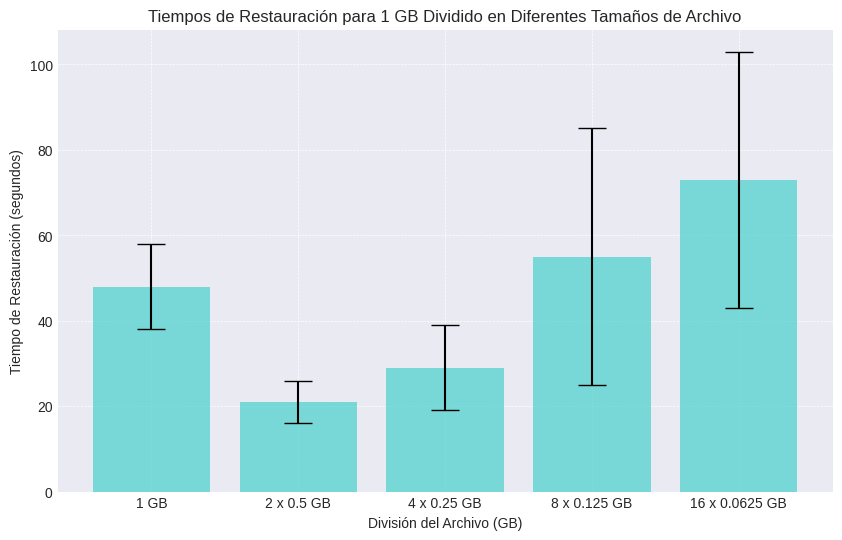
\includegraphics[width=0.8\textwidth]{tiempo_de_restauracion.png}
    \caption{Tiempos de Restauración para 1 GB Dividido en Diferentes Tamaños de Archivo}
    \label{fig:tiempo-restauracion-fraccion}
\end{figure}

\textbf{Descripción de los Datos:}
Los datos muestran que al dividir un archivo de 1 GB en fracciones más pequeñas, el tiempo de restauración varía. Para un solo archivo de 1 GB, el tiempo de restauración es de aproximadamente 48 segundos con una desviación estándar considerable. Cuando se divide en dos archivos de 0.5 GB, el tiempo de restauración disminuye a aproximadamente 21 segundos. Al dividirse en cuatro archivos de 0.25 GB, el tiempo de restauración sube ligeramente a unos 29 segundos. La división en ocho archivos de 0.125 GB resulta en un tiempo de restauración de aproximadamente 55 segundos con una desviación estándar considerable. Finalmente, la división en dieciséis archivos de 0.0625 GB muestra un tiempo de restauración de unos 73 segundos con una desviación estándar también significativa.

\textbf{Análisis de Resultados:}
Los resultados indican que el tiempo de restauración no varía linealmente con la división del archivo de 1 GB en fracciones más pequeñas. La restauración de un archivo grande único o de pocas fracciones grandes tiende a ser más rápida en comparación con la restauración de múltiples fracciones pequeñas. Esto se debe a que la restauración de archivos pequeños implica más operaciones de entrada y salida, así como mayor sobrecarga administrativa, lo que incrementa el tiempo total de restauración.



 %%%%%%%%%%%%%%%


  \subsection{Resultados del Uso de Recursos durante el Backup}

En este apartado se presentan los resultados obtenidos al medir el uso de recursos (CPU y memoria) durante la ejecución de un job de backup, comparado con el uso de recursos en estado baseline. La Figura \ref{fig:uso-recursos} muestra el uso de CPU y memoria en el cliente y el servidor antes y durante la ejecución del job de backup.

\begin{figure}[H]
    \centering
    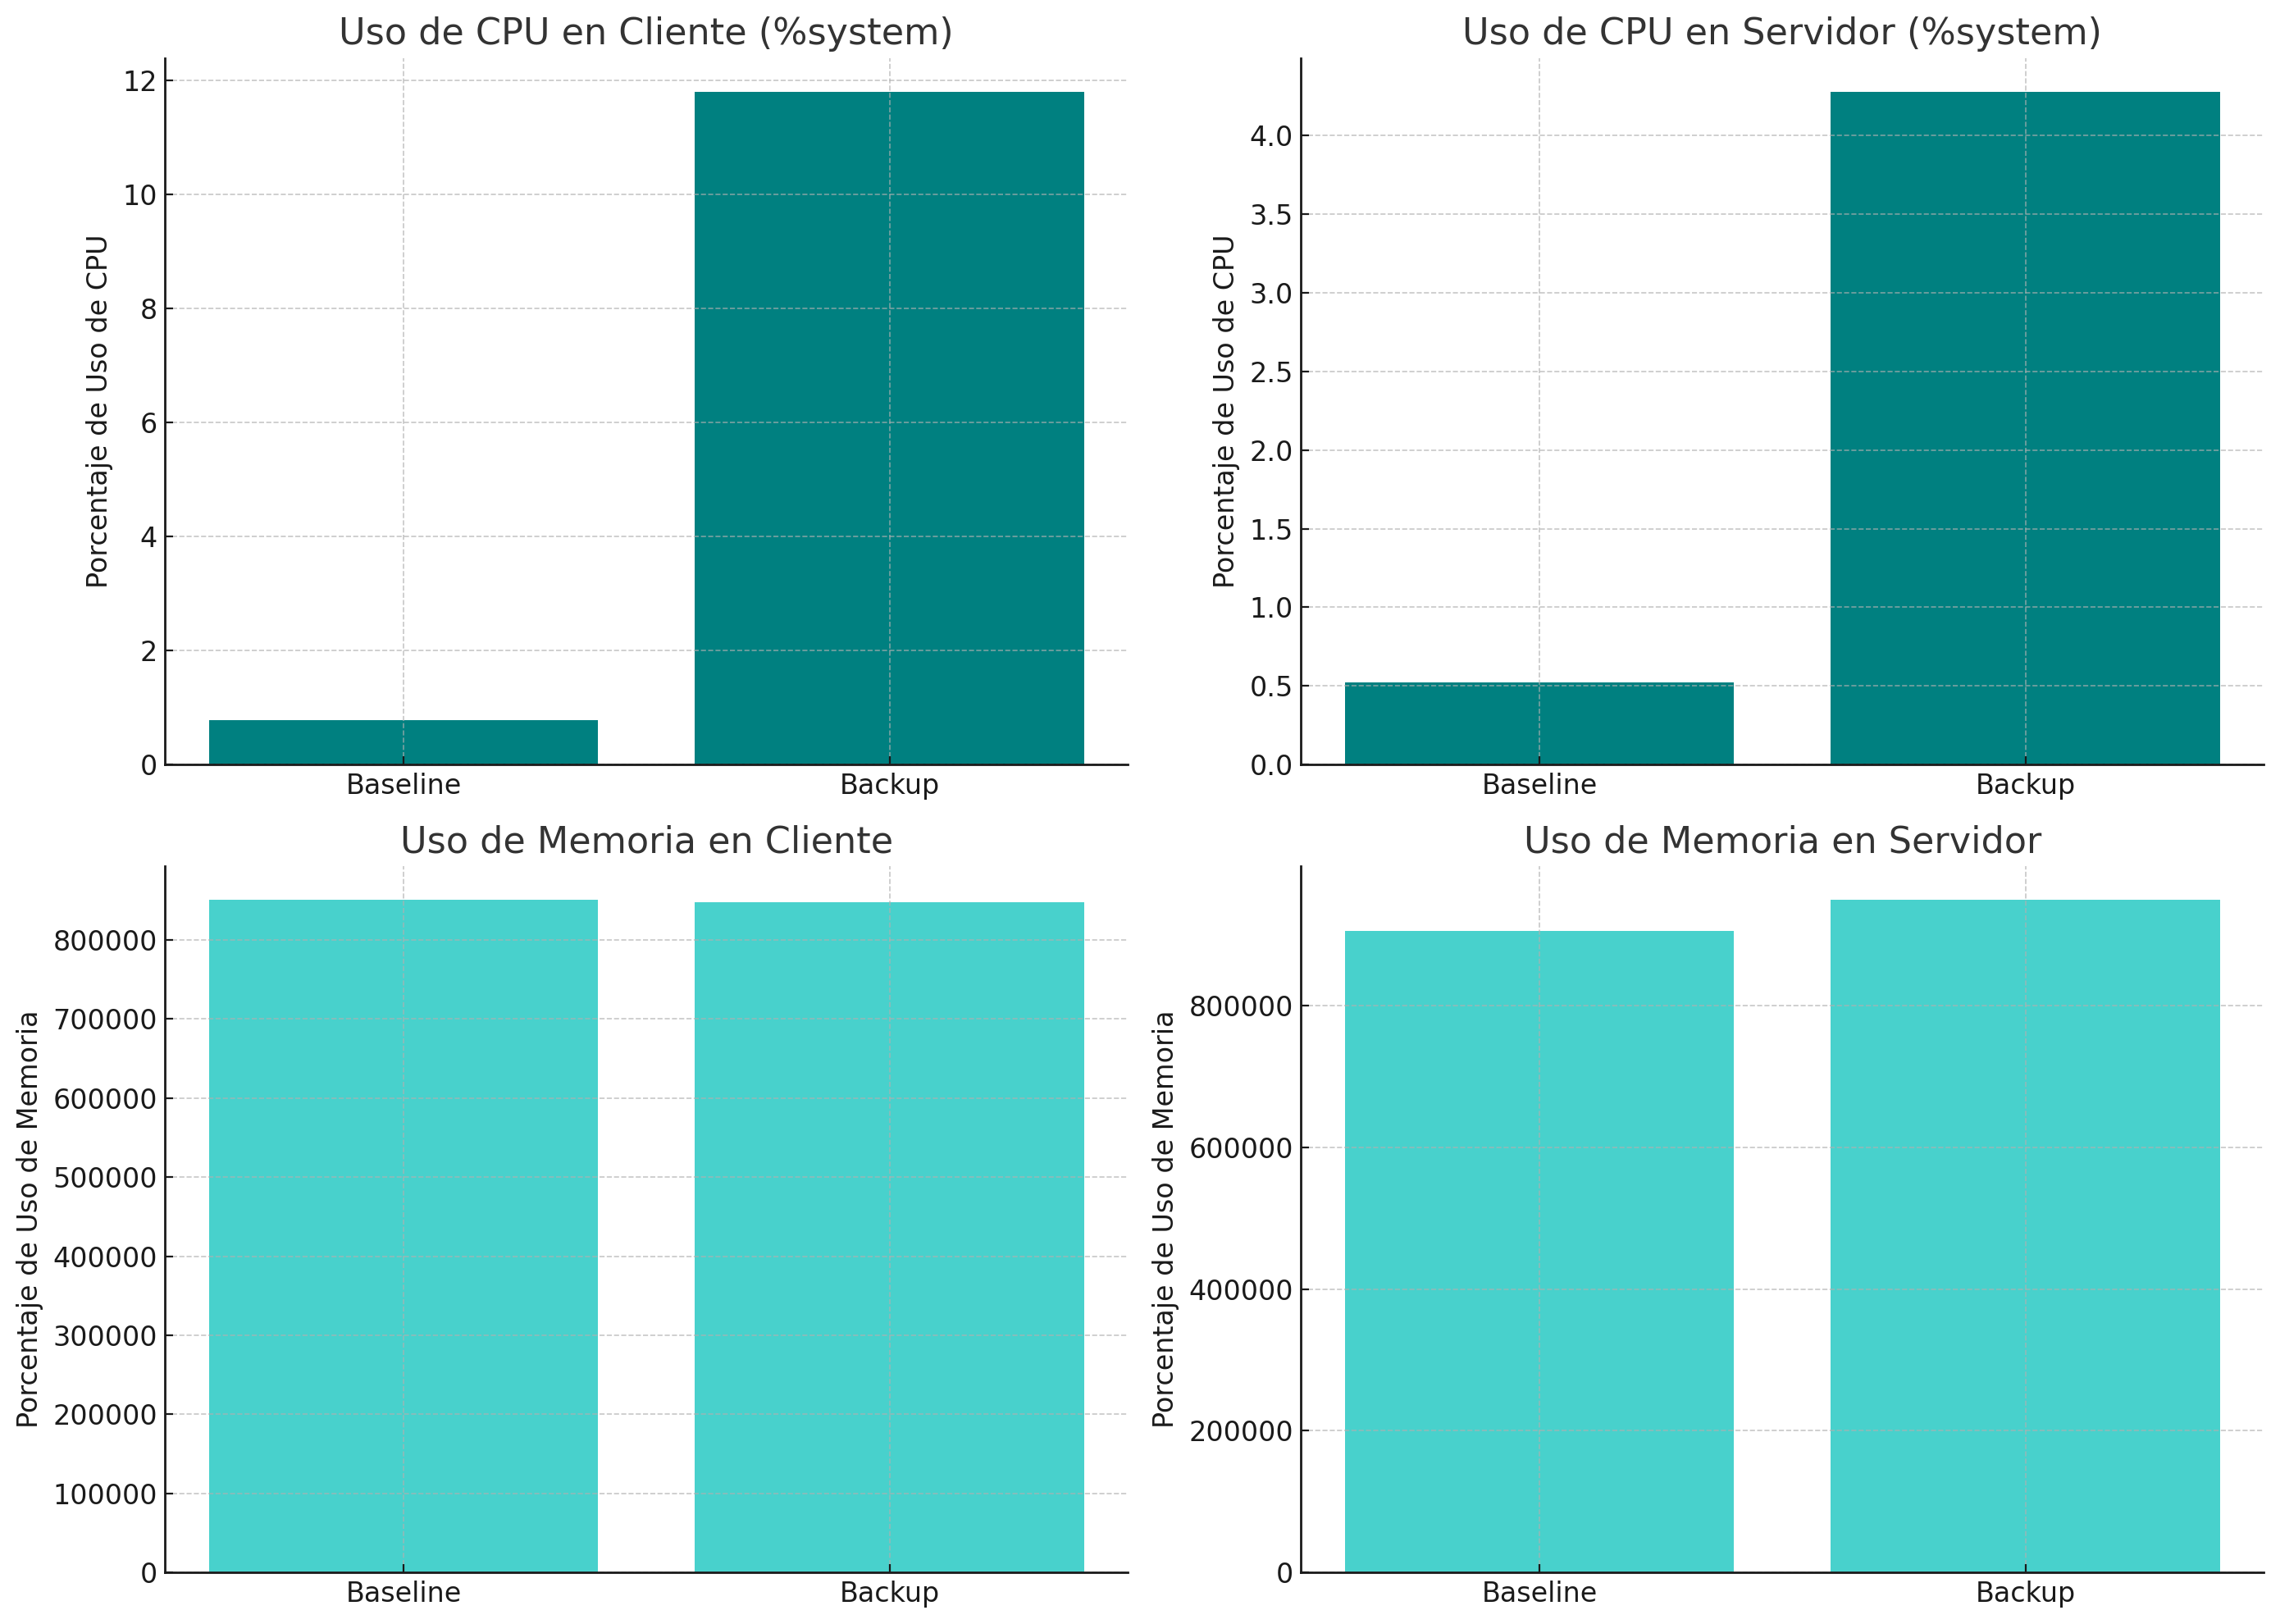
\includegraphics[width=0.8\textwidth]{uso_de_recursos.png}
    \caption{Uso de Recursos durante el Backup}
    \label{fig:uso-recursos}
\end{figure}

\textbf{Descripción de los Datos:}
Los gráficos muestran el uso de CPU (\%system) y memoria en el cliente y en el servidor en dos condiciones: estado baseline y durante el backup.

\textbf{Uso de CPU en el Cliente:}
- En estado baseline, el uso de CPU (\%system) es bajo, alrededor del 1\%.
- Durante el backup, el uso de CPU (\%system) aumenta al 12\%.

\textbf{Uso de CPU en el Servidor:}
- En estado baseline, el uso de CPU (\%system) es alrededor del 0.5\%.
- Durante el backup, el uso de CPU (\%system) se incrementa al 4\%.

\textbf{Uso de Memoria en el Cliente:}
- En estado baseline, el uso de memoria es aproximadamente 820,000 KB.
- Durante el backup, el uso de memoria se mantiene casi constante en aproximadamente 820,000 KB.

\textbf{Uso de Memoria en el Servidor:}
- En estado baseline, el uso de memoria es alrededor de 820,000 KB.
- Durante el backup, el uso de memoria también se mantiene constante en alrededor de 820,000 KB.

\textbf{Análisis de Resultados:}
Los resultados indican que, aunque hay un incremento notable en el uso de CPU (\%system) tanto en el cliente como en el servidor durante el backup, el uso de memoria se mantiene prácticamente constante. Esto sugiere que Bacula, aunque intensivo en el uso de CPU durante los procesos de backup, es eficiente en términos de uso de memoria.
\smallskip
A pesar del incremento en el uso de CPU durante el backup, Bacula utiliza relativamente pocos recursos en comparación con su funcionalidad. El aumento en el uso de CPU es esperado debido a la naturaleza del procesamiento de datos y la escritura en almacenamiento, pero es manejable dentro de los recursos disponibles del sistema. El uso constante de memoria sugiere que Bacula gestiona eficientemente la carga de trabajo sin causar picos significativos en el consumo de memoria, lo que es beneficioso para la estabilidad del sistema y la ejecución de otras tareas concurrentes.


%%%%%%%%%%%%5%%

\subsection{Resultados del Efecto del Número de Jobs en el Tiempo de Backup de 1 GB}

En este apartado se presentan los resultados obtenidos al medir el tiempo de backup de 1 GB en función del número de jobs. La Figura \ref{fig:efecto-numero-jobs} muestra cómo varía el tiempo de backup a medida que se incrementa el número de jobs simultáneos.

\begin{figure}[H]
    \centering
    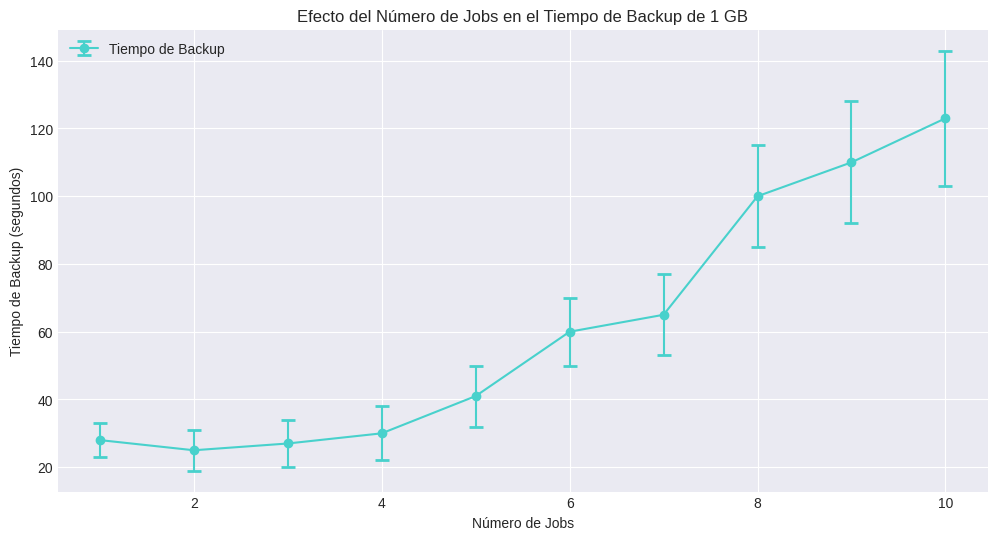
\includegraphics[width=0.8\textwidth]{efecto_numero_jobs.png}
    \caption{Efecto del Número de Jobs en el Tiempo de Backup de 1 GB}
    \label{fig:efecto-numero-jobs}
\end{figure}

\textbf{Descripción de los Datos:}
Los datos muestran que a medida que aumenta el número de jobs simultáneos, el tiempo de backup también incrementa. Con un solo job, el tiempo de backup es de aproximadamente 28 segundos. Cuando se incrementa a dos jobs, el tiempo se mantiene casi constante, pero a partir de cuatro jobs se observa un incremento progresivo en el tiempo de backup, alcanzando aproximadamente 142 segundos con diez jobs.

\textbf{Análisis de Resultados:}
Los resultados indican que hay un punto de inflexión en el cual el incremento del número de jobs comienza a afectar significativamente el tiempo de backup. Hasta cuatro jobs, el tiempo de backup incrementa de manera moderada, pero a partir de seis jobs, el incremento es más pronunciado. Esto sugiere que hay una sobrecarga en el sistema cuando se maneja un alto número de jobs simultáneamente, probablemente debido a la competencia por los recursos del sistema, como la CPU y el I/O de disco.

\textbf{Comportamiento Observado:}
El incremento en el tiempo de backup con el número de jobs puede explicarse por la limitación de los recursos del sistema. Cada job adicional compite por los mismos recursos, lo que puede causar congestión y aumentar el tiempo necesario para completar cada backup. Este comportamiento es consistente con lo esperado en sistemas donde los recursos son compartidos y limitados.






\subsection{Resultados de la Estabilidad Temporal de Tiempos de Backup de 1 GB cada 2 Minutos}

En este apartado se presentan los resultados obtenidos al medir la estabilidad temporal de los tiempos de backup para un archivo de 1 GB realizado cada 2 minutos durante un período de 9 horas y 16 minutos. La Figura \ref{fig:estabilidad-temporal} muestra los tiempos de backup en función del tiempo transcurrido.

\begin{figure}[H]
    \centering
    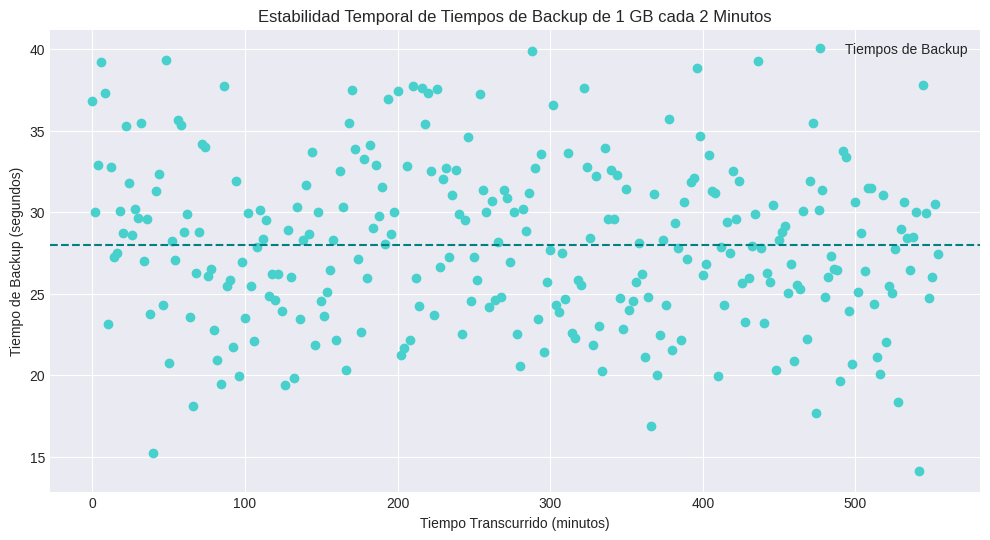
\includegraphics[width=0.8\textwidth]{estabilidad_temporal.png}
    \caption{Estabilidad Temporal de Tiempos de Backup de 1 GB cada 2 Minutos}
    \label{fig:estabilidad-temporal}
\end{figure}

\textbf{Descripción de los Datos:}
Los datos muestran los tiempos de backup de 1 GB medidos cada 2 minutos durante el período de estudio. La gráfica presenta una dispersión de los tiempos de backup alrededor de un valor medio de aproximadamente 28 segundos, con variaciones entre 15 y 40 segundos.

\textbf{Análisis de Resultados:}
Los resultados indican que los tiempos de backup tienen una variabilidad moderada alrededor del valor medio. A lo largo del período de 9 horas y 16 minutos, no se observa una tendencia clara de incremento o decremento en los tiempos de backup, lo que sugiere una estabilidad temporal razonable. La línea punteada en la gráfica representa el valor medio de los tiempos de backup, proporcionando una referencia visual para evaluar la dispersión de los datos.

\textbf{Comportamiento Observado:}
La dispersión de los tiempos de backup puede atribuirse a variaciones en la carga del sistema y en el rendimiento de los recursos compartidos durante el período de estudio. Factores como la actividad de otros procesos, la fluctuación en el rendimiento del almacenamiento y las condiciones de red pueden influir en los tiempos de backup observados. Sin embargo, la falta de una tendencia clara sugiere que el sistema de backup mantiene una consistencia razonable en sus tiempos de operación bajo las condiciones de prueba.


\subsection{Costes de implementación de la Estrategia 3-2-1 en Bacula}

En este apartado se describe la implementación de la estrategia 3-2-1 junto con la estrategia GFS en Bacula, aplicada en la empresa donde trabajo. En esta empresa, utilizamos alrededor de 2 GB mensuales de backup. La implementación se realizará usando un servidor local, una unidad de cinta y almacenamiento en la nube.

\textbf{Tres copias de datos:}
\begin{itemize}
    \item \textbf{Copia 1:} Servidor local.
    \item \textbf{Copia 2:} Cinta.
    \item \textbf{Copia 3:} Nube.
\end{itemize}




\textbf{Cálculo del Almacenamiento Necesario}
\begin{itemize}
    \item \textbf{Cantidad de datos generados:}
    \begin{itemize}
        \item Datos mensuales: 2GB.
        \item Datos anuales: 2GB * 12 meses = 24GB.
        \item Datos en 5 años: 24GB * 5 años = 120GB.
        \item Con un 20\% de margen = 150GB.
    \end{itemize}

    \item \textbf{Estrategia GFS:}
    \begin{itemize}
        \item Backups diarios (incrementales): se retienen aproximadamente 1 semana.
        \item Backups semanales (diferenciales): se retienen aproximadamente 1 mes.
        \item Backups mensuales (completos): se retienen aproximadamente 5 años.
    \end{itemize}
\end{itemize}

Para los cálculos, asumimos que los incrementales y diferenciales son una fracción del tamaño de los completos.

\textbf{Implementación}
\begin{enumerate}
    \item \textbf{Servidor Local}
    \begin{itemize}
        \item \textbf{Hardware:} Servidor con almacenamiento (Fujitsu Primergy Server TX1310 M5 Intel Xeon E-2324G/8GB/2TB).
        \item \textbf{RAID:} 2TB (considerando crecimiento futuro y espacio para snapshots, logs, etc.).
        \item \textbf{Memoria RAM:} 8GB.
    \end{itemize}
    \textbf{Costos aproximados:}
    \begin{itemize}
        \item Servidor: €986,58 \footnote{https://www.pccomponentes.com/fujitsu-primergy-server-tx1310-m5-intel-xeon-e-2324g-8gb-2tb}.
        \item Coste de electricidad: 209 W con un consumo eléctrico de 5.016 kWh y un coste total de €0.25 diarios.
    \end{itemize}

    \item \textbf{Unidad de Cinta}
    \begin{itemize}
        \item \textbf{Hardware:} Unidad de cinta LTO.
    \end{itemize}
    \textbf{Costos aproximados:}
    \begin{itemize}
        \item Unidad LTO: en torno a los €2000.
        \item Cintas LTO (12TB): €50 cada una.
    \end{itemize}

    \item \textbf{Almacenamiento en la Nube}
    \begin{itemize}
        \item \textbf{Proveedor de nube:} AWS S3, Google Cloud Storage, Azure Blob Storage.
    \end{itemize}
    \textbf{Costos aproximados:}
    \begin{itemize}
        \item Costo por almacenamiento en la nube (150GB): Aproximadamente €0.023/GB al mes.
    \end{itemize}
\end{enumerate}

\textbf{Resumen de Costos:}
\begin{itemize}
    \item \textbf{Servidor Local:}
    \begin{itemize}
        \item Costo inicial del servidor: €986,58.
        \item Costo anual de electricidad: €0.25 * 365 = €91.25.
    \end{itemize}
    \item \textbf{Unidad de Cinta:}
    \begin{itemize}
        \item Costo inicial de la unidad LTO: aproximadamente €2000.
        \item Costo de cintas LTO: Asumiendo un total de 150GB, necesitaríamos 1 cintas , lo que sería  €50.
    \end{itemize}
    \item \textbf{Almacenamiento en la Nube:}
    \begin{itemize}
        \item Costo mensual: 150GB * €0.023 = €3.45.
        \item Costo anual: €3.45 * 12 = €41.4.
    \end{itemize}
\end{itemize}

La implementación de la estrategia 3-2-1 junto con la estrategia GFS en Bacula, aunque implica un costo inicial considerable para el hardware y el almacenamiento, asegura la redundancia y la seguridad de los datos. Esta estrategia garantiza que los datos estén protegidos contra fallos del sistema, desastres y otros eventos imprevistos, ofreciendo una solución robusta y fiable para la gestión de backups en la empresa.








